
\section{Unendlichkeit}


% \subsection{Kardinalzahlen}
% 
% \begin{frame}[c]{Kardinalzahlen}
%     \Large
%     Nur zur Differenzierung
% \end{frame}



% \subsection{Ordinalzahlen}



\begin{frame}[c]{Unendlichkeit allgemein}
    \Large
    Unterschied:
    \pause
    \begin{itemize}
        \item Abzählbar Unendlich \only<4->{($\mathbb{N}, \mathbb{Z}, \mathbb{Q}$)}
            \pause
        \item Überabzählbar Unendlich \only<4->{($\mathbb{R}$)}
    \end{itemize}
\end{frame}



\begin{frame}[c]{Problem des Ordinalen Zahlenstrahls}
    \large
    \only<1> {Normaler Zahlenstrahl: \\}
    \only<2> {Normaler Zahlenstrahl mit ersten Ordinalen Zahlen:\\}
    \Huge
    \only<1> {
        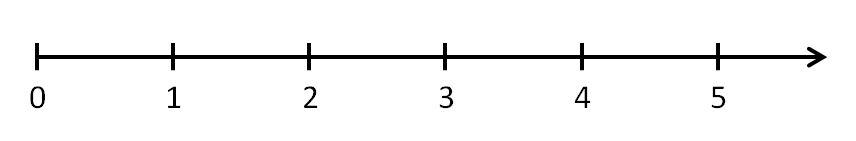
\includegraphics[width=0.8\textwidth]{proseminar/images/zahlenstrahl.jpeg}
        % ganz Normaler Zahlenstrahl, soweit bekannt
        % Zahlen haben Ordinale Eigenschaften
        % Eigenschaften:
        % - Immer entweder Größer, Kleiner oder Gleich
        % - Transitivität
        % - Existenz von Größtem Element in Endlicher Menge
        % Zahlen gehen bis zu unendlich. 
        % Frage nach nach dem Ende des Zahlenstrahls
    }

    \only<2> {
        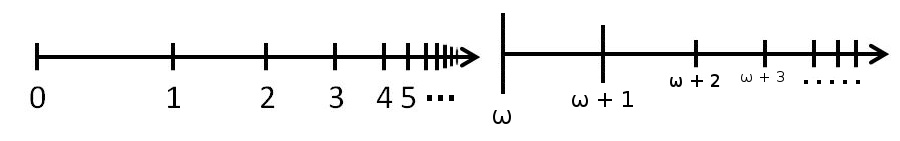
\includegraphics[width=0.85\textwidth]{proseminar/images/zahlenstrahl_ordinal.jpeg}
        % Tadaa! Wir haben zum einen alle 'Normalen' Schritte, haben aber
        % danach immernoch weitere! Wir haben sogar noch Weitere Schritte danach!
    }

    \only<3> {
        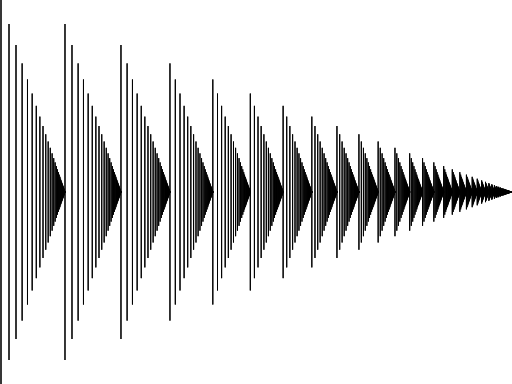
\includegraphics[width=\textwidth]{proseminar/images/ordinal-omega-squared}
        % Das hört da natürlich noch nicht auf, es gibt natürlich noch weitere
        % Stufen, also weitere (explizite) Ordinalzahlen.
        % Bei $\omega * 2$ haben wir also schon 2 mal bis unendlich gezählt!
    }

    \only<4> {
        \hspace{2cm}
        
\includegraphics[height=0.8\textheight]{proseminar/images/ordinal}
        % Es ist so bisschen schwierig das in einen Sinnvollen Zahlenstrahl zu
        % packen ... aber ich hoffe ihr habt verstanden was gemeint ist :)
    }

\end{frame}



